\subsection{2D CNN model}
The initial condition for the 2D problem is a Gaussian function with a standard deviation of 0.1 and a mean of 0.5.
The initial condition can be seen in \autoref{fig:2D_gauss_initial_condition}.
\begin{figure}[H]
    \centering
    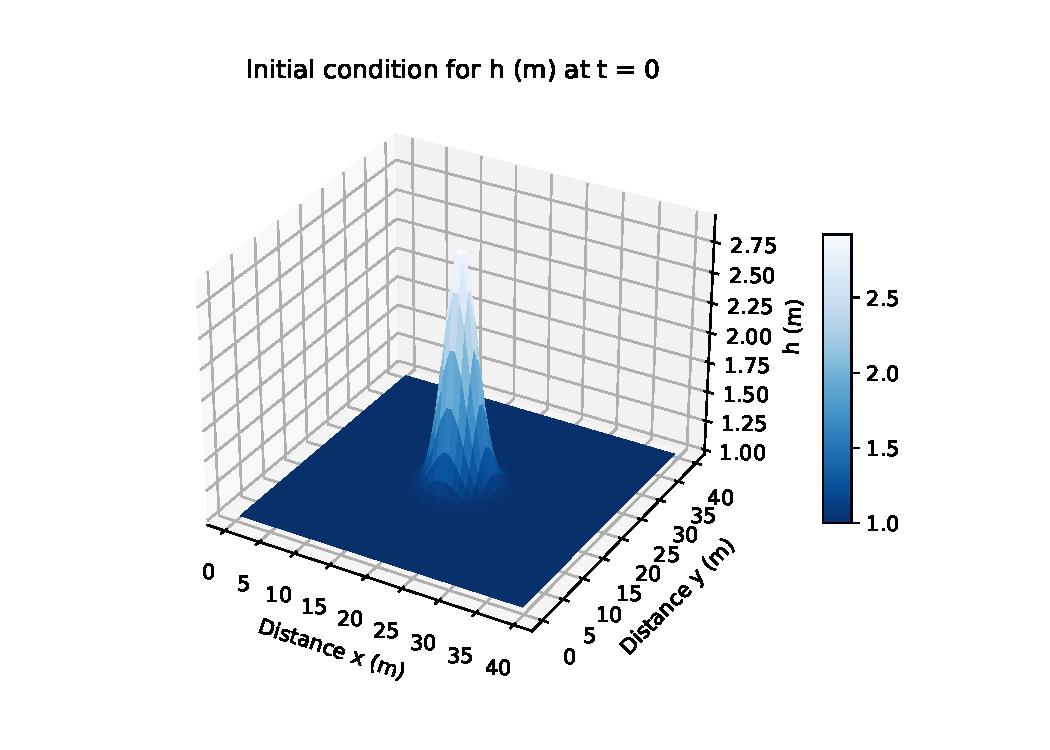
\includegraphics[width=0.8\textwidth]{C:/Users/Matteo/Shallow-Water-Equations/plots/2D_gauss_initial_condition.pdf}
    \caption{Initial condition for the 2D problem.}\label{fig:2D_gauss_initial_condition}
\end{figure}

The training and validation loss for the 2D CNN model can be seen in \autoref{fig:2D_CNN_loss}.
\begin{figure}[H]
    \centering
    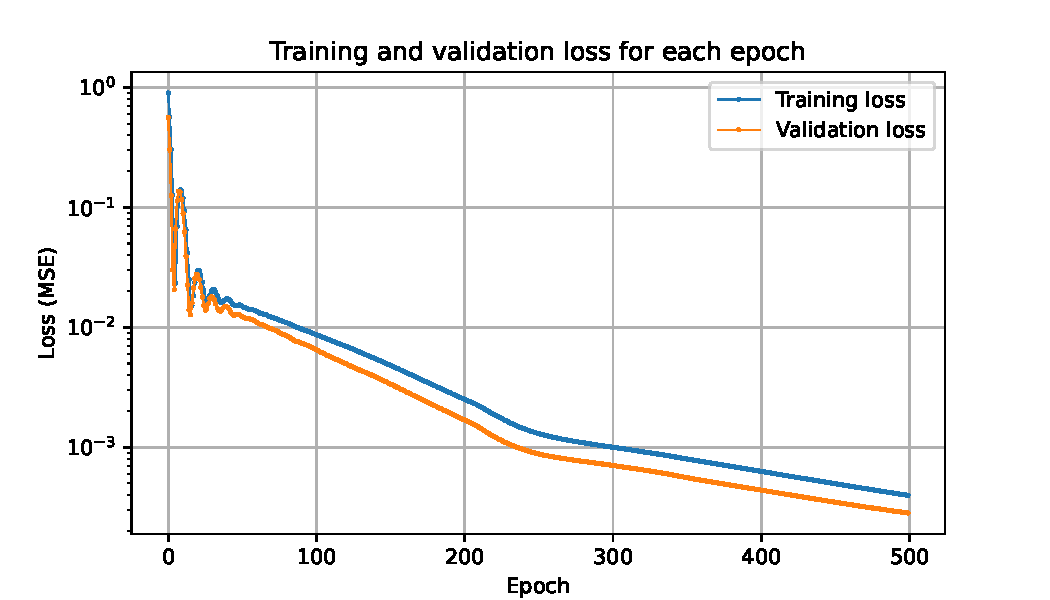
\includegraphics[width=0.7\textwidth]{C:/Users/Matteo/Shallow-Water-Equations/plots/2D_CNN_loss.pdf}
    \caption{Training and validation loss for the 2D CNN model.}\label{fig:2D_CNN_loss}
\end{figure}

The error plot for the last prediction for the 2D CNN can be seen in \autoref{fig:2D_CNN_error}.
\begin{figure}[H]
    \centering
    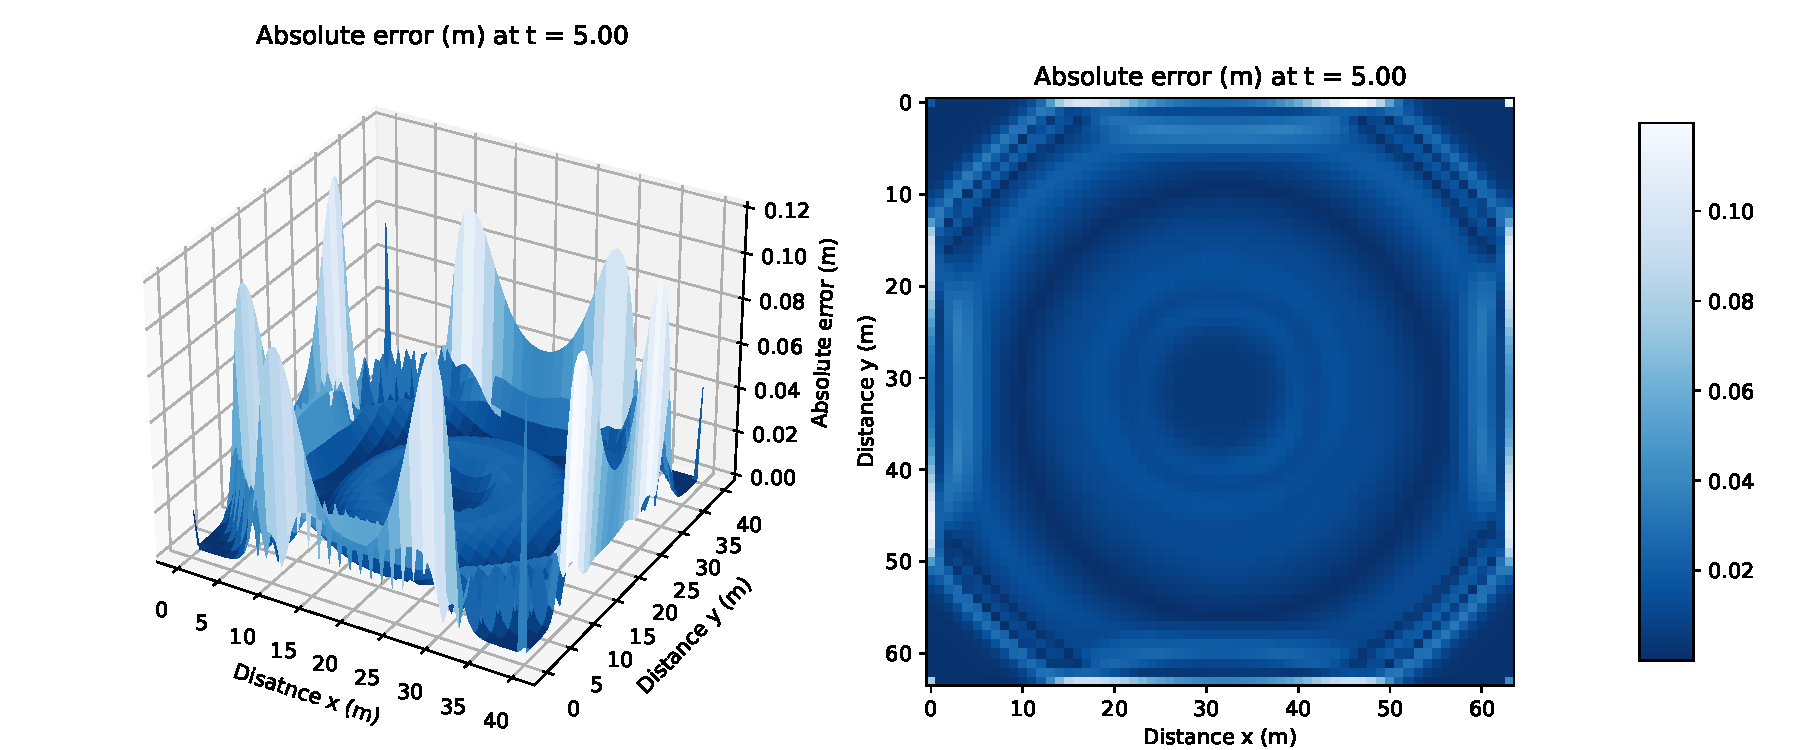
\includegraphics[width=0.8\textwidth]{C:/Users/Matteo/Shallow-Water-Equations/plots/2D_CNN_error.pdf}
    \caption{Error plot for the last prediction for the 2D CNN.}\label{fig:2D_CNN_error}
\end{figure}

\subsection{2D FNO Model}

The training and validation loss for the 2D FNO model can be seen in \autoref{fig:2D_FNO_loss}.
\begin{figure}[H]
    \centering
    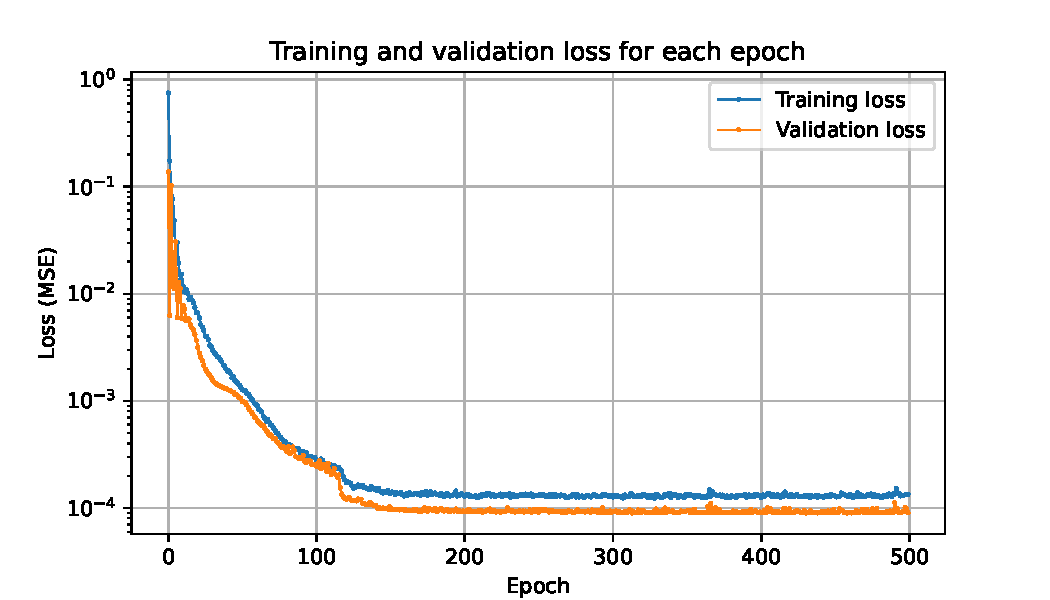
\includegraphics[width=0.8\textwidth]{C:/Users/Matteo/Shallow-Water-Equations/plots/2D_FNO_loss.pdf}
    \caption{Training and validation loss for the 2D FNO model.}\label{fig:2D_FNO_loss}
\end{figure}

The error plot for the last prediction for the 2D FNO can be seen in \autoref{fig:2D_FNO_error}.
\begin{figure}[H]
    \centering
    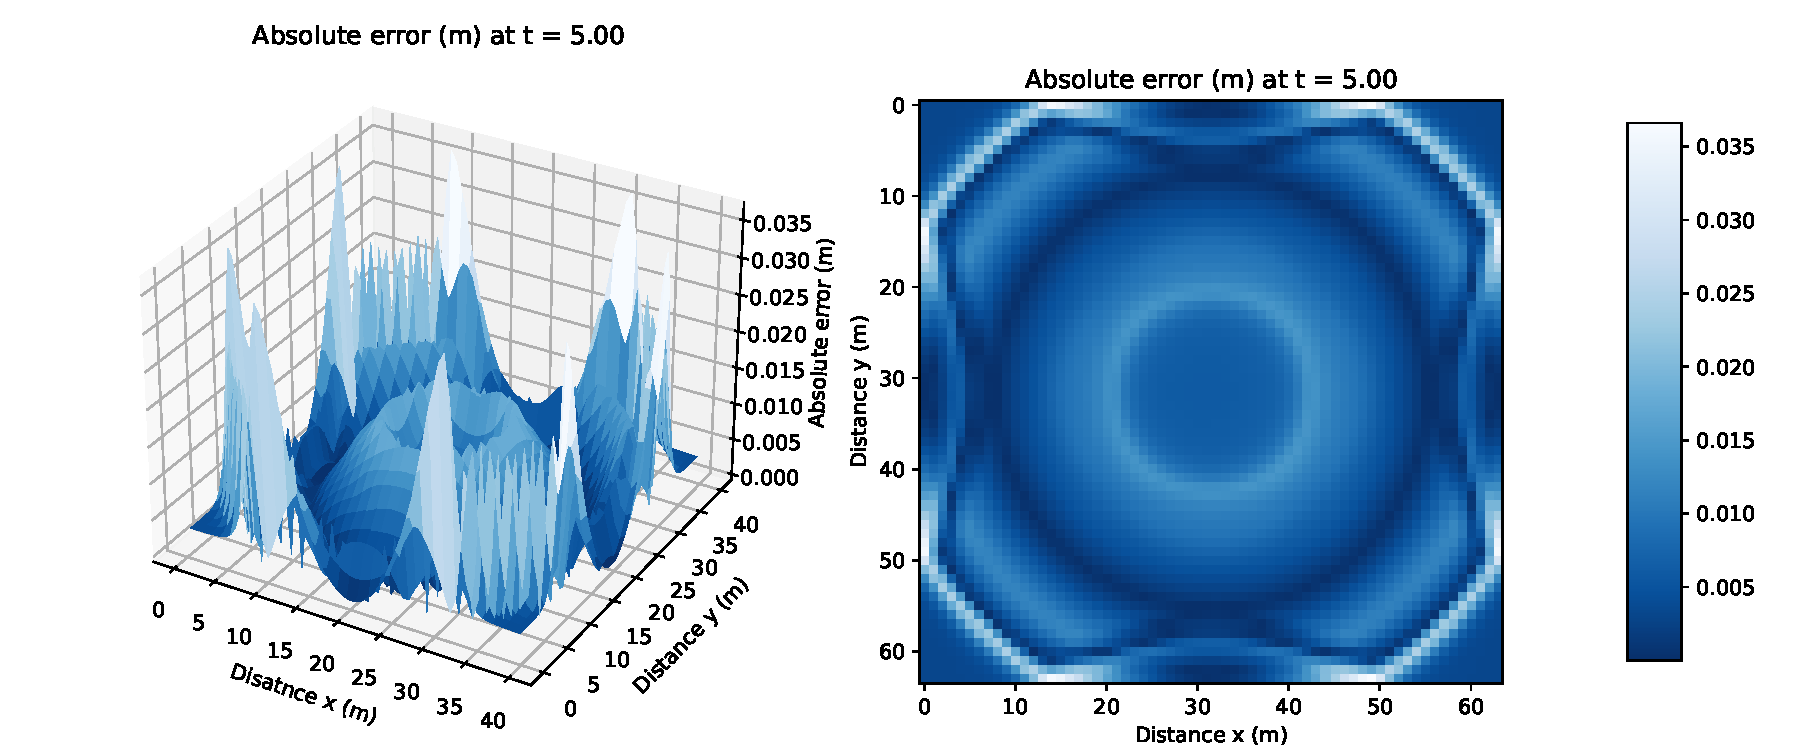
\includegraphics[width=0.8\textwidth]{C:/Users/Matteo/Shallow-Water-Equations/plots/2D_FNO_error.pdf}
    \caption{Error plot for the last prediction for the 2D FNO.}\label{fig:2D_FNO_error}
\end{figure}

\subsection{Comparison between 2D CNN and 2D FNO}


To get an overview of the performance of the different models, we consider the MSE and MAE for the predictions for the 2D SWE case.
\begin{table}[H]
    \centering
    \small % Reduce font size
    \begin{tabular}{c|cccc|cccc}
        Model & \multicolumn{4}{c|}{$N = 50$} & \multicolumn{4}{c}{$N = 100$} \\
        \cline{2-9}
        & Epochs & MSE & MAE & Time (s) & Epochs & MSE & MAE & Time (s) \\
        \hline
        CNN  &
        \input{C:/Users/Matteo/Shallow-Water-Equations/saved_results/2D_CNN_Nx=50_nepochs.txt} &
        \input{C:/Users/Matteo/Shallow-Water-Equations/saved_results/2D_CNN_Nx=50_MSE_test.txt} & 
        \input{C:/Users/Matteo/Shallow-Water-Equations/saved_results/2D_CNN_Nx=50_MAE_test.txt} &
        \input{C:/Users/Matteo/Shallow-Water-Equations/saved_results/2D_CNN_Nx=50_time.txt} &
        \input{C:/Users/Matteo/Shallow-Water-Equations/saved_results/2D_CNN_Nx=100_nepochs.txt} &
        \input{C:/Users/Matteo/Shallow-Water-Equations/saved_results/2D_CNN_Nx=100_MSE_test.txt} &
        \input{C:/Users/Matteo/Shallow-Water-Equations/saved_results/2D_CNN_Nx=100_MAE_test.txt} &
        \input{C:/Users/Matteo/Shallow-Water-Equations/saved_results/2D_CNN_Nx=100_time.txt} 
        \\
        \hline
        FNO  &
        \input{C:/Users/Matteo/Shallow-Water-Equations/saved_results/2D_FNO_Nx=50_nepochs.txt} &
        \input{C:/Users/Matteo/Shallow-Water-Equations/saved_results/2D_FNO_Nx=50_MSE_test.txt} &
        \input{C:/Users/Matteo/Shallow-Water-Equations/saved_results/2D_FNO_Nx=50_MAE_test.txt} &
        \input{C:/Users/Matteo/Shallow-Water-Equations/saved_results/2D_FNO_Nx=50_time.txt} &
        \input{C:/Users/Matteo/Shallow-Water-Equations/saved_results/2D_CNN_Nx=100_nepochs.txt} &
        \input{C:/Users/Matteo/Shallow-Water-Equations/saved_results/2D_FNO_Nx=100_MSE_test.txt} &
        \input{C:/Users/Matteo/Shallow-Water-Equations/saved_results/2D_FNO_Nx=100_MAE_test.txt} &
        \input{C:/Users/Matteo/Shallow-Water-Equations/saved_results/2D_FNO_Nx=100_time.txt}
        \\
        \hline
    \end{tabular}
    \caption{Test loss in terms of MSE and MAE, and time for training the models for the 2D SWE.}\label{tab:results_2D_comparison}
\end{table}

We see that the FNO model in general needs fewer epochs to converge compared to the CNN model, but it also takes longer time to train.
Try with a new initial condition? 


